% Provenance (never printed): cycle 4 SVT, "La planete Terre, l'environnement
% et l'action humaine": the relief as a balance between uplift and erosion;
% landforms of the wind, the sea and dissolution; reading a landscape; see
% sources/book1/PROVENANCE.md. Book 1, grade 9, chapter 4.
% Vocabulary guard: owns uplift, dune, cliff, beach and spit (with longshore
% drift), karst (with cave and sinkhole). Landscape and landform are g1's;
% weathering, erosion, deposition, meander and delta are g5's; relief is
% g4's; plates and mountain building are g7's; U-shaped valley and moraine
% are g8's; limestone and the acid test are g6's; acids are the chemistry
% books' (recalled in prose). Contour lines are g9.5's (not used here).
% "Normal fault" and the destruction of mountains are Book 2's.
\chapter{地貌}\label{ch:g9:landforms}

英格兰南\omterm{def:g1:landscapes-around-us:water}{海岸}的七姐妹白色\omterm{def:g9:landforms:cliff}{悬崖}，
直接落入大海。在正常年份里，它们最多后退一米。
2014 年冬天，\omterm{def:g5:natural-hazards:storm}{风暴}从伯林盖普的\omterm{def:g9:landforms:cliff}{悬崖}上带走的岩体，
相当于它们平时七年的损失量，却只用了两个月。这些\omterm{def:g9:landforms:cliff}{悬崖}的白垩
曾是海底的\omterm{def:g3:stones-pebbles-sand:sand}{淤泥}，由生活在海水中的微观藻类的细小板状骨骼构成。
如今它矗立成一道白色岩壁，
海浪每年都让它再后退一点。为什么大地会有如今的形态？
其中一些\omterm{def:g1:landscapes-around-us:landform}{地貌}为何变化得如此之快？
% ledger: nt:birling-2014, sdnp:birling, nasa:coccoliths

\begin{omfigure}
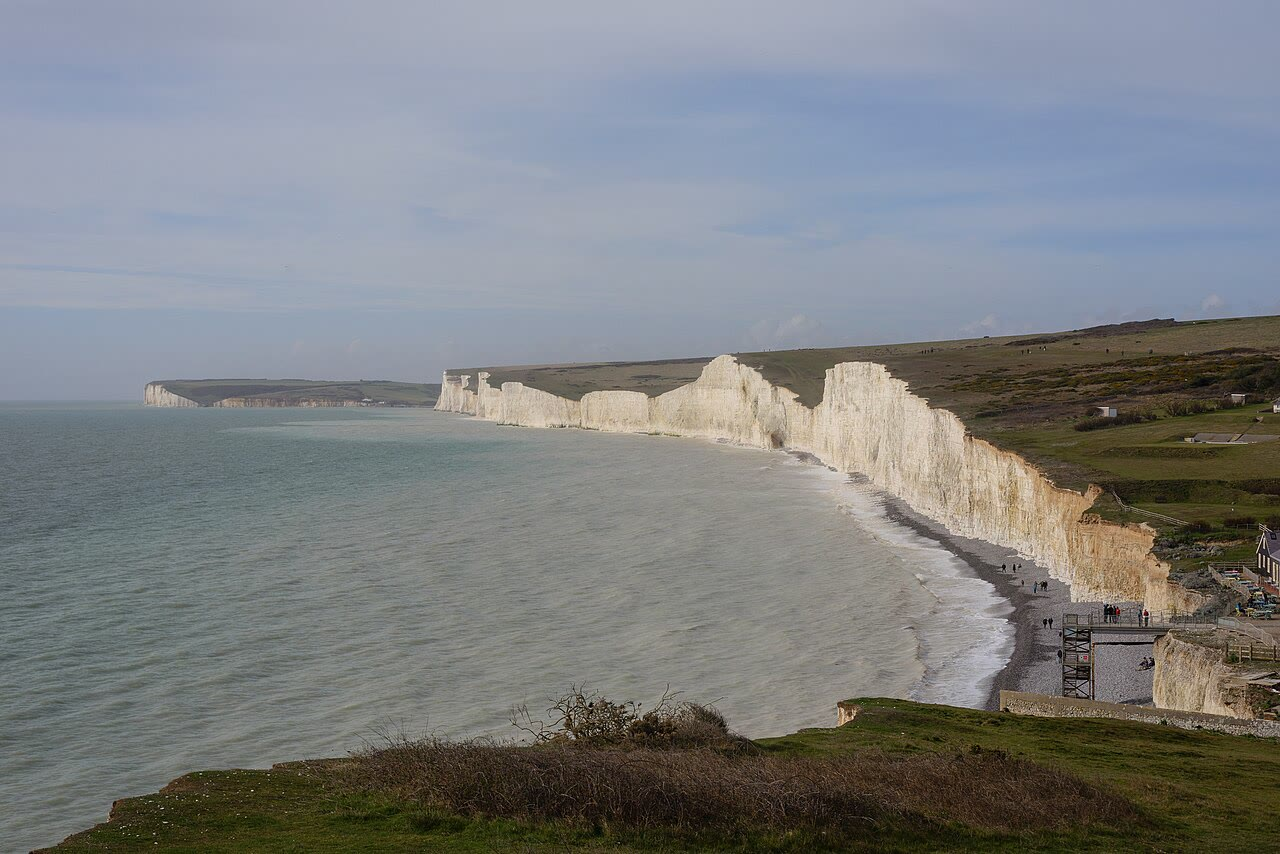
\includegraphics[width=\linewidth]{images/book1/g9-seven-sisters.jpg}

{\small 七姐妹，英格兰东萨塞克斯郡\omterm{def:g1:landscapes-around-us:water}{海岸}的白垩\omterm{def:g9:landforms:cliff}{悬崖}，
前景为伯林盖普的房屋。\omterm{def:g9:landforms:cliff}{悬崖}不断受海浪\omterm{def:g5:water-shapes-the-land:erosion}{侵蚀}，
\omterm{def:g3:stones-pebbles-sand:rock}{岩石}崩塌随时可能发生。\omterm{def:g9:landforms:cliff}{悬崖}脚下是一片
\omterm{def:g3:stones-pebbles-sand:pebble}{卵石}\omterm{def:g9:landforms:beach}{海滩}。照片：Arild Vågen, 2017（CC BY-SA 4.0，经
维基共享资源）。}
% ledger: commons:seven-sisters, sdnp:birling
\label{fig:g9:landforms:seven-sisters}
\end{omfigure}

\begin{recall}
\emph{\omterm{def:g1:landscapes-around-us:landform}{地貌}}是地表形态的一种，如\omterm{def:g1:landscapes-around-us:landform}{丘陵}、\omterm{def:g1:landscapes-around-us:landform}{山谷}、\omterm{def:g1:landscapes-around-us:landform}{平原}、
\omterm{def:g9:landforms:cliff}{悬崖}（\cref{ch:g1:landscapes-around-us}）。\omterm{def:g4:world-physical-map:relief}{地形起伏}是地表
高度的分布（\cref{ch:g4:world-physical-map}）。\omterm{def:g5:water-shapes-the-land:weathering}{风化}使\omterm{def:g3:stones-pebbles-sand:rock}{岩石}破碎，
\omterm{def:g5:water-shapes-the-land:erosion}{侵蚀}将其磨损并搬走，\omterm{def:g5:water-shapes-the-land:deposition}{沉积}则将其堆积于别处
（\cref{ch:g5:water-shapes-the-land}）。板块在碰撞处挤压，
抬升形成\omterm{def:g4:world-physical-map:range}{山脉}（\cref{ch:g7:plate-tectonics}）；\omterm{def:g8:ice-on-earth:glacier}{冰川}\omterm{def:g5:water-shapes-the-land:erosion}{侵蚀}出 \omterm{def:g8:ice-on-earth:glacial-landforms}{U 形谷}
（\cref{ch:g8:ice-on-earth}）；石灰岩遇
稀酸即起泡（\cref{ch:g6:rocks-and-minerals}）。在化学中，你会学到
酸会与石灰岩反应，并放出二氧化碳。
\end{recall}

\section{地形起伏：隆升与侵蚀的平衡}

塑造\omterm{def:g4:world-physical-map:relief}{地形起伏}的力有两类。来自内部的
板块运动抬升地面。来自外部的水、冰、风与海，
则不断将其磨损。

\begin{definition}[隆升]\label{def:g9:landforms:uplift}
\emph{隆升}\index{隆升}是某一地区的\omterm{def:g3:stones-pebbles-sand:rock}{岩石}和地表缓慢上升的过程，
由地球内部的力驱动，
例如两个板块的碰撞。
\end{definition}

以生命的尺度看，\omterm{def:g9:landforms:uplift}{隆升}很慢；以地球的尺度看，它却很快。
印度约在 5000 万年前与亚洲碰撞，喜马拉雅山北侧的
青藏高原获得了大部分高度，约
\qty{4600}{m}，主要在最近 1000 万年内获得。平均
下来相当于 $4600 \div 10^7 = 4.6 \times 10^{-4}$~m，即每年约 \qty{0.5}{mm}：
比指甲的厚度还小，但持续数百万年便十分可观。
% ledger: usgs:himalaya (rate computed in figdata/grade-9/cliff_retreat.py, tibet_rate_mm_yr)

地面一旦抬升，\omterm{def:g5:water-shapes-the-land:erosion}{侵蚀}便随之而来。地势越高、坡度越陡，
\omterm{def:g1:landscapes-around-us:water}{河流}、\omterm{def:g8:ice-on-earth:glacier}{冰川}和岩崩搬走\omterm{def:g3:stones-pebbles-sand:rock}{岩石}的速度就越快，
\omterm{def:g4:world-physical-map:range}{山脉}在任一时刻的高度，是一场角力的结果：
\omterm{def:g9:landforms:uplift}{隆升}所抬高的，减去\omterm{def:g5:water-shapes-the-land:erosion}{侵蚀}所带走的。

\begin{omfigure}
\begin{tikzpicture}[font=\footnotesize, >={Stealth[length=2mm]}]
  % panel 1: uplift faster than erosion
  \begin{scope}
    \fill[black!13] (0,0) -- (0.5,0) .. controls (1.1,1.0) and (1.5,2.0) .. (1.8,2.2)
      .. controls (2.1,2.0) and (2.5,1.0) .. (3.1,0) -- (3.6,0) -- (3.6,-0.5) -- (0,-0.5) -- cycle;
    \draw[black!60] (0,0) -- (0.5,0) .. controls (1.1,1.0) and (1.5,2.0) .. (1.8,2.2)
      .. controls (2.1,2.0) and (2.5,1.0) .. (3.1,0) -- (3.6,0);
    \draw[black!60, dashed] (0.7,0) .. controls (1.2,0.8) and (1.5,1.5) .. (1.8,1.6)
      .. controls (2.1,1.5) and (2.4,0.8) .. (2.9,0);
    \foreach \x in {1.2,1.8,2.4} \draw[->, omWarm, line width=1.4pt] (\x,-0.45) -- ++(0,1.0);
    \draw[->, omRiver, thick] (2.15,1.6) -- ++(0.35,-0.3);
    \node[align=center, anchor=north] at (1.8,-0.6) {隆升快于侵蚀：\\地势升高};
  \end{scope}
  % panel 2: uplift equals erosion
  \begin{scope}[xshift=4.4cm]
    \fill[black!13] (0,0) -- (0.5,0) .. controls (1.1,1.0) and (1.5,1.8) .. (1.8,1.9)
      .. controls (2.1,1.8) and (2.5,1.0) .. (3.1,0) -- (3.6,0) -- (3.6,-0.5) -- (0,-0.5) -- cycle;
    \draw[black!60] (0,0) -- (0.5,0) .. controls (1.1,1.0) and (1.5,1.8) .. (1.8,1.9)
      .. controls (2.1,1.8) and (2.5,1.0) .. (3.1,0) -- (3.6,0);
    \foreach \x in {1.2,1.8,2.4} \draw[->, omWarm, line width=1.4pt] (\x,-0.45) -- ++(0,0.6);
    \draw[->, omRiver, thick] (2.05,1.6) -- ++(0.55,-0.5);
    \draw[->, omRiver, thick] (1.55,1.6) -- ++(-0.55,-0.5);
    \node[align=center, anchor=north] at (1.8,-0.6) {隆升与侵蚀相等：\\地势高度保持不变};
  \end{scope}
  % panel 3: no more uplift
  \begin{scope}[xshift=8.8cm]
    \fill[black!13] (0,0) -- (0.4,0) .. controls (1.1,0.5) and (1.5,0.95) .. (1.8,1.0)
      .. controls (2.1,0.95) and (2.5,0.5) .. (3.2,0) -- (3.6,0) -- (3.6,-0.5) -- (0,-0.5) -- cycle;
    \draw[black!60] (0,0) -- (0.4,0) .. controls (1.1,0.5) and (1.5,0.95) .. (1.8,1.0)
      .. controls (2.1,0.95) and (2.5,0.5) .. (3.2,0) -- (3.6,0);
    \draw[black!60, dashed] (0.5,0) .. controls (1.1,1.0) and (1.5,1.8) .. (1.8,1.9)
      .. controls (2.1,1.8) and (2.5,1.0) .. (3.1,0);
    \draw[->, omRiver, thick] (2.05,0.95) -- ++(0.55,-0.5);
    \draw[->, omRiver, thick] (1.55,0.95) -- ++(-0.55,-0.5);
    \node[align=center, anchor=north] at (1.8,-0.6) {不再隆升：侵蚀 \\使地势降低};
  \end{scope}
  % key
  \draw[->, omWarm, line width=1.4pt] (13.2,1.2) -- ++(0,0.6) node[right, black] {隆升};
  \draw[->, omRiver, thick] (13.2,0.7) -- ++(0.35,-0.3) node[right, black] {侵蚀};
  \draw[black!60, dashed] (13.1,-0.1) -- ++(0.5,0) node[right, black] {早先剖面};
\end{tikzpicture}

{\small \omterm{def:g4:world-physical-map:relief}{地形起伏}作为一种平衡（示意图，不按比例）。\omterm{def:g9:landforms:uplift}{隆升}抬高
\omterm{def:g3:stones-pebbles-sand:rock}{岩石}；\omterm{def:g5:water-shapes-the-land:erosion}{侵蚀}将其搬运至\omterm{def:g1:landscapes-around-us:landform}{山谷}与海中。\omterm{def:g4:world-physical-map:range}{山脉}
只要\omterm{def:g9:landforms:uplift}{隆升}占优便持续增高；板块停止推挤后，\omterm{def:g5:water-shapes-the-land:erosion}{侵蚀}便缓慢地
将其磨蚀为\omterm{def:g1:landscapes-around-us:landform}{丘陵}。}
\label{fig:g9:landforms:balance}
\end{omfigure}

\omterm{def:g1:landscapes-around-us:water}{河流}（\cref{ch:g5:water-shapes-the-land}）和\omterm{def:g8:ice-on-earth:glacier}{冰川}
（\cref{ch:g8:ice-on-earth}）是雕刻\omterm{def:g4:world-physical-map:range}{山脉}的主要力量。本章其余部分
将讨论另外三种各自塑造\omterm{def:g1:landscapes-around-us:landform}{地貌}的营力，
即风、海，以及溶解\omterm{def:g3:stones-pebbles-sand:rock}{岩石}的水。

\section{风力作用形成的地貌：沙丘}

在植物稀少、松散\omterm{def:g3:stones-pebbles-sand:sand}{沙子}丰富且风力强劲的地方，风
可卷起\omterm{def:g3:stones-pebbles-sand:sand}{沙子}并堆积成丘，常见于\omterm{def:g5:weather-and-climate:desert}{沙漠}，以及沙质
\omterm{def:g9:landforms:beach}{海滩}的后方。
% ledger: nps:aeolian

\begin{definition}[沙丘]\label{def:g9:landforms:dune}
称\emph{沙丘}\index{沙丘}为由风堆积起来的松散\omterm{def:g3:stones-pebbles-sand:sand}{沙子}形成的
丘状或脊状堆积体。其迎风坡长而缓；背风一侧，即
\emph{滑落面}\index{滑落面}，短而陡。
\end{definition}
% ledger: nps:aeolian, nmt:barchan

\omterm{def:g9:landforms:dune}{沙丘}会移动。风将\omterm{def:g3:stones-pebbles-sand:sand}{沙粒}沿缓坡滚动和跳跃上推；
在坡顶，\omterm{def:g3:stones-pebbles-sand:sand}{沙粒}不断堆积，直至堆积体过陡，
一小股沙崩便沿\omterm{def:g9:landforms:dune}{滑落面}滑下。\omterm{def:g3:stones-pebbles-sand:sand}{沙粒}一粒接一粒，\omterm{def:g3:stones-pebbles-sand:sand}{沙子}
自迎风一侧被搬走，堆积在背风一侧，整个\omterm{def:g9:landforms:dune}{沙丘}
向下风方向缓慢爬行，却从不被整体抬起。\omterm{def:g9:landforms:dune}{沙丘}很少单独存在：它们
常常覆盖大片区域。
% ledger: nmt:barchan, nps:aeolian

当风向始终一致且沙量不太多时，\omterm{def:g9:landforms:dune}{沙丘}呈新月形，即
\emph{巴尔汗\omterm{def:g9:landforms:dune}{沙丘}}：圆钝的一端迎风，
两翼则指向下风方向。两翼所含\omterm{def:g3:stones-pebbles-sand:sand}{沙子}比中部少，
因而移动更快，并向\omterm{def:g9:landforms:dune}{沙丘}前方伸展。
% ledger: nmt:barchan

\begin{omfigure}
\begin{tikzpicture}[font=\footnotesize, >={Stealth[length=2mm]}]
  % plan view
  \fill[yellow!25!orange!20] (3.4,1.3) .. controls (1.0,1.3) and (0.2,0.6) .. (0.2,0)
     .. controls (0.2,-0.6) and (1.0,-1.3) .. (3.4,-1.3)
     .. controls (2.4,-0.9) and (1.8,-0.5) .. (1.8,0)
     .. controls (1.8,0.5) and (2.4,0.9) .. (3.4,1.3) -- cycle;
  \fill[orange!45] (3.4,1.3) .. controls (2.4,0.9) and (1.8,0.5) .. (1.8,0)
     .. controls (1.8,-0.5) and (2.4,-0.9) .. (3.4,-1.3)
     .. controls (2.1,-0.8) and (1.45,-0.45) .. (1.45,0)
     .. controls (1.45,0.45) and (2.1,0.8) .. (3.4,1.3) -- cycle;
  \draw[black!60] (3.4,1.3) .. controls (1.0,1.3) and (0.2,0.6) .. (0.2,0)
     .. controls (0.2,-0.6) and (1.0,-1.3) .. (3.4,-1.3)
     .. controls (2.4,-0.9) and (1.8,-0.5) .. (1.8,0)
     .. controls (1.8,0.5) and (2.4,0.9) .. (3.4,1.3);
  \draw[black, thick] (3.4,1.3) .. controls (2.1,0.8) and (1.45,0.45) .. (1.45,0)
     .. controls (1.45,-0.45) and (2.1,-0.8) .. (3.4,-1.3);
  \foreach \y in {-0.8,0,0.8} \draw[->, omRiver, thick] (-1.3,\y) -- ++(1.1,0);
  \node[above] at (-0.75,0.85) {风};
  \node[anchor=west] at (3.5,1.35) {角};
  \node[anchor=west] at (3.5,-1.35) {角};
  \draw[black!70] (1.75,0.25) -- (2.9,0.35) node[anchor=west, align=left, black] {滑落面 \\（陡）};
  \draw[black!70] (0.75,-0.2) -- (0.6,-1.6) node[anchor=north, align=center, black] {迎风坡 \\（缓）};
  \draw[black!70] (1.47,-0.3) -- (2.4,-1.75) node[anchor=north, black] {坡顶};
  \node[anchor=south, font=\footnotesize\bfseries] at (1.4,1.6) {俯视};
  % profile
  \begin{scope}[xshift=7.2cm, yshift=-0.8cm]
    \draw[black!60] (-0.4,0) -- (5.6,0);
    \fill[yellow!25!orange!20] (0,0) -- (3.0,1.2) -- (3.6,0) -- cycle;
    \draw[black!70] (0,0) -- (3.0,1.2) -- (3.6,0);
    \fill[orange!45] (3.0,1.2) -- (3.6,0) -- (3.3,0) -- cycle;
    \draw[black!50, dashed] (0.8,0) -- (3.8,1.2) -- (4.4,0);
    \draw[->, black!70] (0.5,0.35) .. controls (0.75,0.65) .. (1.0,0.45);
    \draw[->, black!70] (1.0,0.55) .. controls (1.25,0.85) .. (1.5,0.65);
    \draw[->, black!70] (1.5,0.75) .. controls (1.75,1.05) .. (2.0,0.85);
    \draw[->, black!70] (2.0,0.95) .. controls (2.25,1.25) .. (2.5,1.05);
    \draw[->, thick, black!80] (3.15,1.05) -- (3.45,0.35);
    \foreach \y in {1.6,2.1} \draw[->, omRiver, thick] (-0.8,\y) -- ++(1.1,0);
    \node[above] at (-0.25,2.1) {风};
    \draw[->, thick] (4.5,0.6) -- ++(0.7,0) node[right, align=left] {沙丘 \\移动};
    \node[align=center, anchor=north] at (1.2,-0.1) {沙粒沿缓坡 \\跳跃上升};
    \node[align=center, anchor=north west] at (2.9,-0.1) {然后沿滑落面 \\滑下};
    \node[anchor=south, font=\footnotesize\bfseries] at (2.2,2.3) {侧视};
  \end{scope}
\end{tikzpicture}

{\small 新月形\omterm{def:g9:landforms:dune}{沙丘}，即巴尔汗\omterm{def:g9:landforms:dune}{沙丘}（示意图）。俯视时，其两翼
指向下风方向。侧视时，\omterm{def:g3:stones-pebbles-sand:sand}{沙粒}沿缓慢的迎风坡
向上爬升，再沿陡峭的\omterm{def:g9:landforms:dune}{滑落面}滑下：\omterm{def:g9:landforms:dune}{沙丘}向下风方向移动（虚线
为稍后时刻的\omterm{def:g9:landforms:dune}{沙丘}轮廓）。}
% ledger: nmt:barchan, nps:aeolian
\label{fig:g9:landforms:barchan}
\end{omfigure}

移动有多快？在新墨西哥州白沙国家公园的石膏\omterm{def:g9:landforms:dune}{沙丘}区中，
在其迎风边缘形成的小\omterm{def:g9:landforms:dune}{沙丘}，高仅数米，每年最快可移动
\qty{6}{m}；再往前，长到 6 至 \qty{10}{m} 高的\omterm{def:g9:landforms:dune}{沙丘}，
它们每年约移动 \qty{3}{m}。\omterm{def:g9:landforms:dune}{沙丘}积沙越多，
移动越慢。由强风驱动的巴尔汗\omterm{def:g9:landforms:dune}{沙丘}可移动超过 \qty{100}{m}，
一年内足以掩埋一条道路或一片田地。
% ledger: nps:whsa-migration, nmt:barchan

\begin{omfigure}
\begin{minipage}[c]{0.5\linewidth}\centering
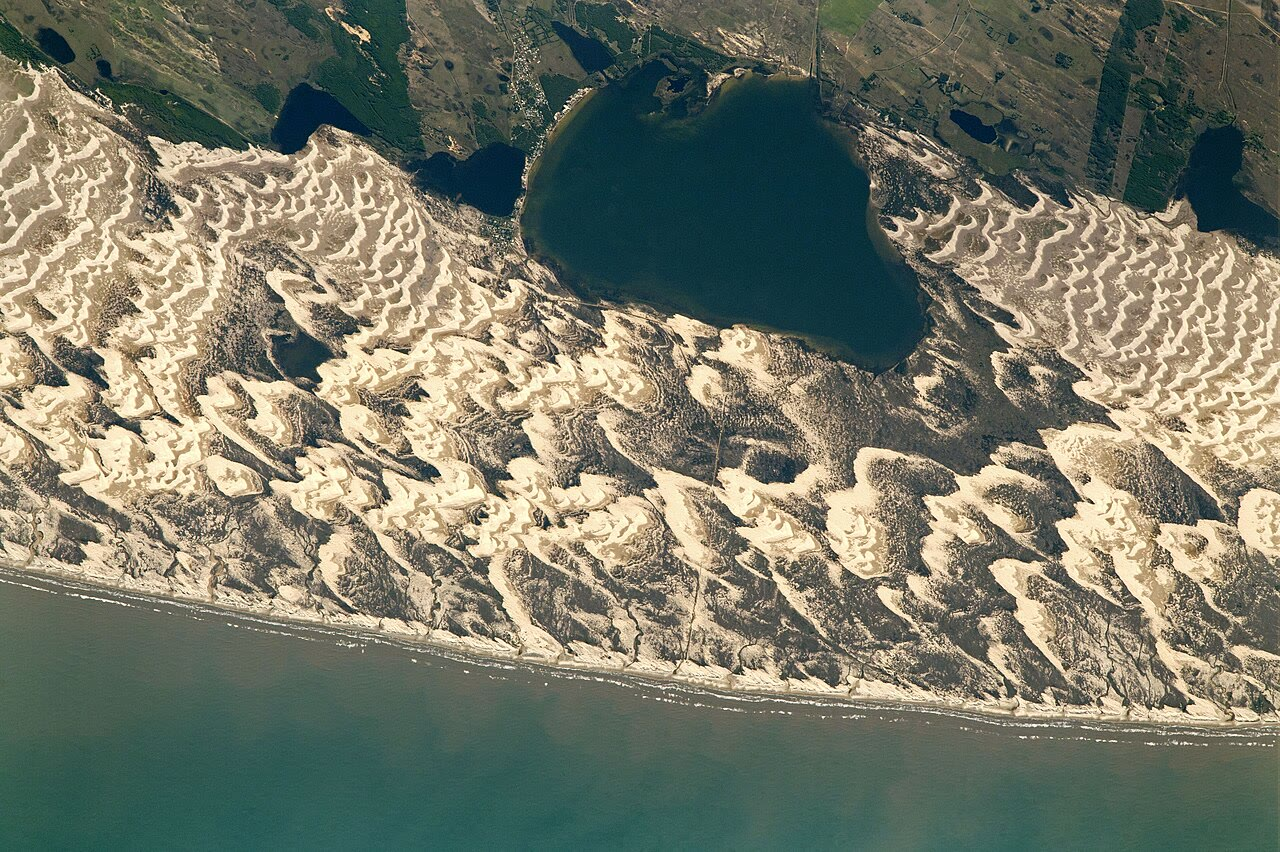
\includegraphics[width=\linewidth]{images/book1/g9-barchans.jpg}
\end{minipage}\hfill
\begin{minipage}[c]{0.46\linewidth}\raggedright
{\small 巴西南部大西洋\omterm{def:g1:landscapes-around-us:water}{海岸}的新月形\omterm{def:g9:landforms:dune}{沙丘}，
2017 年由宇航员从国际空间站拍摄。
暗色的巴罗斯湖（Lagoa dos Barros）长约 \qty{4.5}{km}。\omterm{def:g3:stones-pebbles-sand:sand}{沙子}
来自照片底部的\omterm{def:g9:landforms:beach}{海滩}。NASA（公有领域，
经维基共享资源）。}
\end{minipage}
% ledger: commons:iss-barchans
\label{fig:g9:landforms:barchans-photo}
\end{omfigure}

\omterm{def:g1:landscapes-around-us:water}{海岸}上，\omterm{def:g9:landforms:beach}{海滩}后方的一排\omterm{def:g9:landforms:dune}{沙丘}保护着其后的陆地
免受\omterm{def:g5:natural-hazards:storm}{风暴}浪的侵袭。生长在\omterm{def:g9:landforms:dune}{沙丘}上的植物用根
固定住\omterm{def:g3:stones-pebbles-sand:sand}{沙子}：一旦植物被踩踏或清除，风又会把\omterm{def:g3:stones-pebbles-sand:sand}{沙子}吹走。
% ledger: nps:aeolian

\section{海洋作用形成的地貌}

\subsection{悬崖}

\begin{definition}[悬崖]\label{def:g9:landforms:cliff}
\emph{悬崖}\index{悬崖}是陡峭或竖直的岩壁。在
\omterm{def:g1:landscapes-around-us:water}{海岸}上，悬崖被海浪切割，海浪冲击其底部，使悬崖向内陆
后退。
\end{definition}

海浪将水、沙和\omterm{def:g3:stones-pebbles-sand:pebble}{卵石}抛向\omterm{def:g9:landforms:cliff}{悬崖}底部，逐渐
在崖底切出一个凹槽，即\emph{海蚀凹口}，位于
低潮与高潮水位之间。上方\omterm{def:g3:stones-pebbles-sand:rock}{岩石}向外悬出，雨水和霜冻使其
进一步松动。某日，悬出的岩块崩落。海浪将崩落的岩块打碎并搬走，
\omterm{def:g5:water-shapes-the-land:erosion}{侵蚀}又在新的崖面上开始，位置稍向内陆
推移。其后，\omterm{def:g9:landforms:cliff}{悬崖}留下一个平坦的岩台，即
\emph{海蚀平台}\index{海蚀平台}，在低潮时
露出。
% ledger: nt:birling-2014, sdnp:birling

软岩后退最快。在伯林盖普，白垩\omterm{def:g9:landforms:cliff}{悬崖}每年最多
后退约一米；不过后退是跳跃式的，一次崩落一段，
\omterm{def:g5:natural-hazards:storm}{风暴}频发的冬季可能一次造成数年的后退量。1999 年，旧的
贝勒图特灯塔于 1832 年建于附近\omterm{def:g9:landforms:cliff}{悬崖}顶部，
因崖边逐渐逼近，灯塔整体后移了 \qty{17}{m}，
离开崖缘。
% ledger: sdnp:birling, nt:birling-2014

\begin{omfigure}
\begin{tikzpicture}[font=\footnotesize, >={Stealth[length=2mm]}]
  % panel 1: the notch
  \begin{scope}
    \fill[omSea!45] (0,-0.1) rectangle (1.8,0.75);
    \fill[omSea!45] (1.8,0.35) -- (2.25,0.55) -- (1.8,0.95) -- cycle;
    \fill[black!8] (1.6,-0.1) -- (1.8,0.25) -- (1.8,0.35) -- (2.25,0.55) -- (1.8,0.95) -- (1.8,2.4) -- (3.6,2.4) -- (3.6,-0.6) -- (0,-0.6) -- (0,-0.1) -- cycle;
    \draw[black!70] (0,-0.1) -- (1.6,-0.1) -- (1.8,0.25) -- (1.8,0.35) -- (2.25,0.55) -- (1.8,0.95) -- (1.8,2.4) -- (3.6,2.4);
    \foreach \y in {0.8,1.3,1.8} \draw[black!25] (1.8,\y) -- (3.6,\y);
    \fill[green!35!black!50] (1.8,2.4) rectangle (3.6,2.5);
    \draw[->, omSea!80!black, thick] (0.4,0.6) -- (1.6,0.6);
    \node[anchor=south, align=center] at (0.9,0.8) {海浪};
    \draw[black!70] (2.15,0.55) -- (2.9,1.0) node[anchor=west, fill=white, inner sep=1pt] {海蚀凹口};
    \node[anchor=north, align=center] at (1.8,-0.7) {1. 海浪切出 \\凹口};
    \node[anchor=south, font=\footnotesize] at (2.7,2.5) {白垩};
  \end{scope}
  % panel 2: collapse
  \begin{scope}[xshift=4.6cm]
    \fill[omSea!45] (0,-0.1) rectangle (2.2,0.75);
    \fill[black!8] (2.0,-0.1) -- (2.2,0.25) -- (2.25,2.4) -- (3.6,2.4) -- (3.6,-0.6) -- (0,-0.6) -- (0,-0.1) -- cycle;
    \draw[black!70] (0,-0.1) -- (2.0,-0.1) -- (2.2,0.25) -- (2.25,2.4) -- (3.6,2.4);
    \draw[black!50, dashed] (1.8,0.95) -- (1.8,2.4) -- (2.25,2.4);
    \foreach \y in {0.8,1.3,1.8} \draw[black!25] (2.25,\y) -- (3.6,\y);
    \fill[green!35!black!50] (2.25,2.4) rectangle (3.6,2.5);
    \foreach \x/\y/\s in {1.25/0.05/0.28, 1.6/0.1/0.22, 1.95/0.3/0.3, 1.45/0.35/0.18}
      \fill[black!20, draw=black!60] (\x,\y) rectangle ++(\s,\s*0.8);
    \node[anchor=north, align=center] at (1.8,-0.7) {2. 悬挑岩体 \\崩落};
  \end{scope}
  % panel 3: retreat and platform
  \begin{scope}[xshift=9.2cm]
    \fill[omSea!45] (0,0.2) rectangle (2.8,0.75);
    \fill[black!8] (0,0.0) -- (2.6,0.2) -- (2.8,0.3) -- (2.85,2.4) -- (4.0,2.4) -- (4.0,-0.6) -- (0,-0.6) -- cycle;
    \draw[black!70] (0,0.0) -- (2.6,0.2) -- (2.8,0.3) -- (2.85,2.4) -- (4.0,2.4);
    \foreach \y in {0.8,1.3,1.8} \draw[black!25] (2.85,\y) -- (4.0,\y);
    \fill[green!35!black!50] (2.85,2.4) rectangle (4.0,2.5);
    \draw[black!50, dashed] (1.4,0.12) -- (1.4,2.4);
    \draw[black!50, dashed] (2.1,0.16) -- (2.1,2.4);
    \draw[<-, thick] (2.8,1.6) -- (1.5,1.6);
    \node[anchor=south, align=center] at (1.4,2.45) {旧崖面};
    \node[anchor=north, align=center] at (2.0,-0.7) {3. 海蚀平台，\\低潮时露出};
  \end{scope}
\end{tikzpicture}

{\small 海蚀\omterm{def:g9:landforms:cliff}{悬崖}的后退过程（示意图，未按比例绘制）。（1）海浪
在崖底切出凹口。（2）悬挑岩体崩落；海浪
打碎岩块并将其搬走。（3）循环重复：\omterm{def:g9:landforms:cliff}{悬崖}
向陆地后退，并在其前方留下一个平坦的岩台。}
% ledger: nt:birling-2014, sdnp:birling
\label{fig:g9:landforms:cliff-retreat}
\end{omfigure}

\begin{safety}
\omterm{def:g9:landforms:cliff}{悬崖}边缘随时可能崩塌，岩块也会
毫无预警地从崖面坠落。观察\omterm{def:g9:landforms:cliff}{悬崖}应保持安全距离，
在崖顶远离边缘，在崖下\omterm{def:g9:landforms:beach}{海滩}上远离崖脚，并且
在涨潮前离开\omterm{def:g9:landforms:cliff}{悬崖}下方的\omterm{def:g9:landforms:beach}{海滩}。
\end{safety}
% ledger: nt:birling-2014, sdnp:birling

\subsection{海滩与沙嘴}

从\omterm{def:g9:landforms:cliff}{悬崖}上磨蚀下来、又由\omterm{def:g1:landscapes-around-us:water}{河流}带来的沙和\omterm{def:g3:stones-pebbles-sand:pebble}{卵石}，并不会
停留在落下的地方：海浪对它们进行分选，并沿\omterm{def:g1:landscapes-around-us:water}{海岸}搬运。

\begin{definition}[海滩、沿岸漂移与沙嘴]\label{def:g9:landforms:beach}
\emph{海滩}\index{海滩}是由海浪沿岸堆积起来的
沙或\omterm{def:g3:stones-pebbles-sand:pebble}{卵石}带状堆积体。当海浪以一定角度抵达岸边时，每一个
海浪都沿这一角度将砂粒推上海滩，而水流
则沿坡面直线回落：砂粒便沿\omterm{def:g1:landscapes-around-us:water}{海岸}呈之字形移动。这种
沙和\omterm{def:g3:stones-pebbles-sand:pebble}{卵石}沿\omterm{def:g1:landscapes-around-us:water}{海岸}的运动即\emph{沿岸
漂移}\index{沿岸漂移}。\emph{沙嘴}\index{沙嘴}是狭长的
沙、\omterm{def:g3:stones-pebbles-sand:pebble}{卵石}脊，由沿岸漂移堆积而成，
一端与陆地相连，另一端在\omterm{def:g1:landscapes-around-us:water}{海岸}转折处伸入大海。
\end{definition}
% ledger: noaa:longshore

\omterm{def:g1:landscapes-around-us:water}{海岸}拐弯处，例如海湾口或\omterm{def:g5:water-shapes-the-land:source-mouth}{河口}处，漂移
沿同一方向继续进行，并在较平静的水中卸下所携带的物质：
\omterm{def:g9:landforms:beach}{海滩}便向海中延伸，形成\omterm{def:g9:landforms:beach}{沙嘴}。其末端常向内侧弯曲，
受来自其他方向的海浪影响而弯曲。\omterm{def:g9:landforms:beach}{沙嘴}后方
避开海浪的一侧，泥\omterm{def:g5:water-shapes-the-land:deposition}{沉积}，盐沼发育。
% ledger: noaa:longshore

\begin{omfigure}
\begin{tikzpicture}[font=\footnotesize, >={Stealth[length=2mm]}]
  % sea
  \fill[omSea!40] (0,0) rectangle (11,2.3);
  % land with a bay
  \fill[green!25!black!20] (0,2.3) -- (6,2.3) .. controls (6.3,3.0) and (7.0,3.5) .. (8.0,3.5)
     .. controls (9.0,3.5) and (9.3,2.8) .. (9.5,2.3) -- (11,2.3) -- (11,4.6) -- (0,4.6) -- cycle;
  % calm water of the bay
  \fill[omSea!20] (6,2.3) .. controls (6.3,3.0) and (7.0,3.5) .. (8.0,3.5)
     .. controls (9.0,3.5) and (9.3,2.8) .. (9.5,2.3) -- cycle;
  % salt marsh
  \fill[green!50!black!35] (6.15,2.55) .. controls (6.6,3.1) and (7.3,3.2) .. (7.9,3.0)
     .. controls (7.6,2.7) and (7.0,2.6) .. (6.15,2.55) -- cycle;
  \node[anchor=west, font=\scriptsize] at (6.5,3.85) {盐沼};
  \draw[black!60] (6.9,3.75) -- (7.0,2.95);
  % river
  \draw[omRiver, line width=1.2pt] (8.6,4.6) .. controls (8.5,4.0) and (8.3,3.7) .. (8.3,3.48);
  \node[anchor=west, font=\scriptsize] at (8.65,4.25) {河流};
  % beach
  \fill[yellow!40!orange!35] (0,1.85) rectangle (6,2.3);
  % spit
  \fill[yellow!40!orange!35] (5.9,1.85) .. controls (7.0,1.95) and (7.8,2.0) .. (8.35,2.1)
     .. controls (8.6,2.2) and (8.6,2.5) .. (8.4,2.65) -- (8.25,2.55)
     .. controls (8.35,2.45) and (8.3,2.35) .. (8.15,2.32)
     .. controls (7.5,2.28) and (6.8,2.3) .. (6.0,2.3) -- cycle;
  \draw[black!60] (0,2.3) -- (6,2.3) .. controls (6.3,3.0) and (7.0,3.5) .. (8.0,3.5)
     .. controls (9.0,3.5) and (9.3,2.8) .. (9.5,2.3) -- (11,2.3);
  % waves arriving at an angle
  \foreach \x in {0.9,2.0,3.1,4.2} \draw[omSea!70!black, line width=0.5pt] (\x,1.15) -- ++(-35:1.1);
  \draw[->, omSea!70!black, thick] (0.6,0.3) -- ++(55:1.2) node[pos=0.15, left, black] {海浪};
  % zigzag of a pebble
  \draw[->, black, thick] (1.0,1.9) -- (1.35,2.2) -- (1.35,1.9) -- (1.7,2.2) -- (1.7,1.9)
     -- (2.05,2.2) -- (2.05,1.9) -- (2.4,2.2) -- (2.4,1.9);
  \node[anchor=south, align=center, font=\scriptsize] at (1.7,2.45) {沿海滩斜向冲上 \\然后 \\笔直退回};
  % drift arrow
  \draw[->, line width=1.6pt, omWarm] (3.0,1.55) -- (5.6,1.55) node[midway, below, black] {沿岸漂移};
  % spit label
  \draw[black!70] (7.4,2.05) -- (7.6,1.2) node[anchor=north, align=center, black] {沙嘴横跨 \\海湾生长};
  \draw[->, thick, omWarm] (8.6,1.95) -- ++(0.6,0);
  % compass
  \draw[->] (10.4,0.3) -- ++(0,0.6) node[above] {北};
\end{tikzpicture}

{\small \omterm{def:g9:landforms:beach}{沿岸漂移}与\omterm{def:g9:landforms:beach}{沙嘴}的俯视示意图（略图）。海浪自西南方向而来，
每一次都将沙与\omterm{def:g3:stones-pebbles-sand:pebble}{卵石}斜向推上\omterm{def:g9:landforms:beach}{海滩}，随后水流笔直退回，
颗粒因而之字形地向东移动。\omterm{def:g1:landscapes-around-us:water}{海岸}拐成海湾处，漂移继续进行，
并形成\omterm{def:g9:landforms:beach}{沙嘴}，\omterm{def:g9:landforms:beach}{沙嘴}后方发育盐沼。
\omterm{def:g1:landscapes-around-us:water}{河流}在\omterm{def:g9:landforms:beach}{沙嘴}末端
保持一条河道畅通。}
% ledger: noaa:longshore
\label{fig:g9:landforms:spit}
\end{omfigure}

\begin{omfigure}
\begin{minipage}[c]{0.5\linewidth}\centering
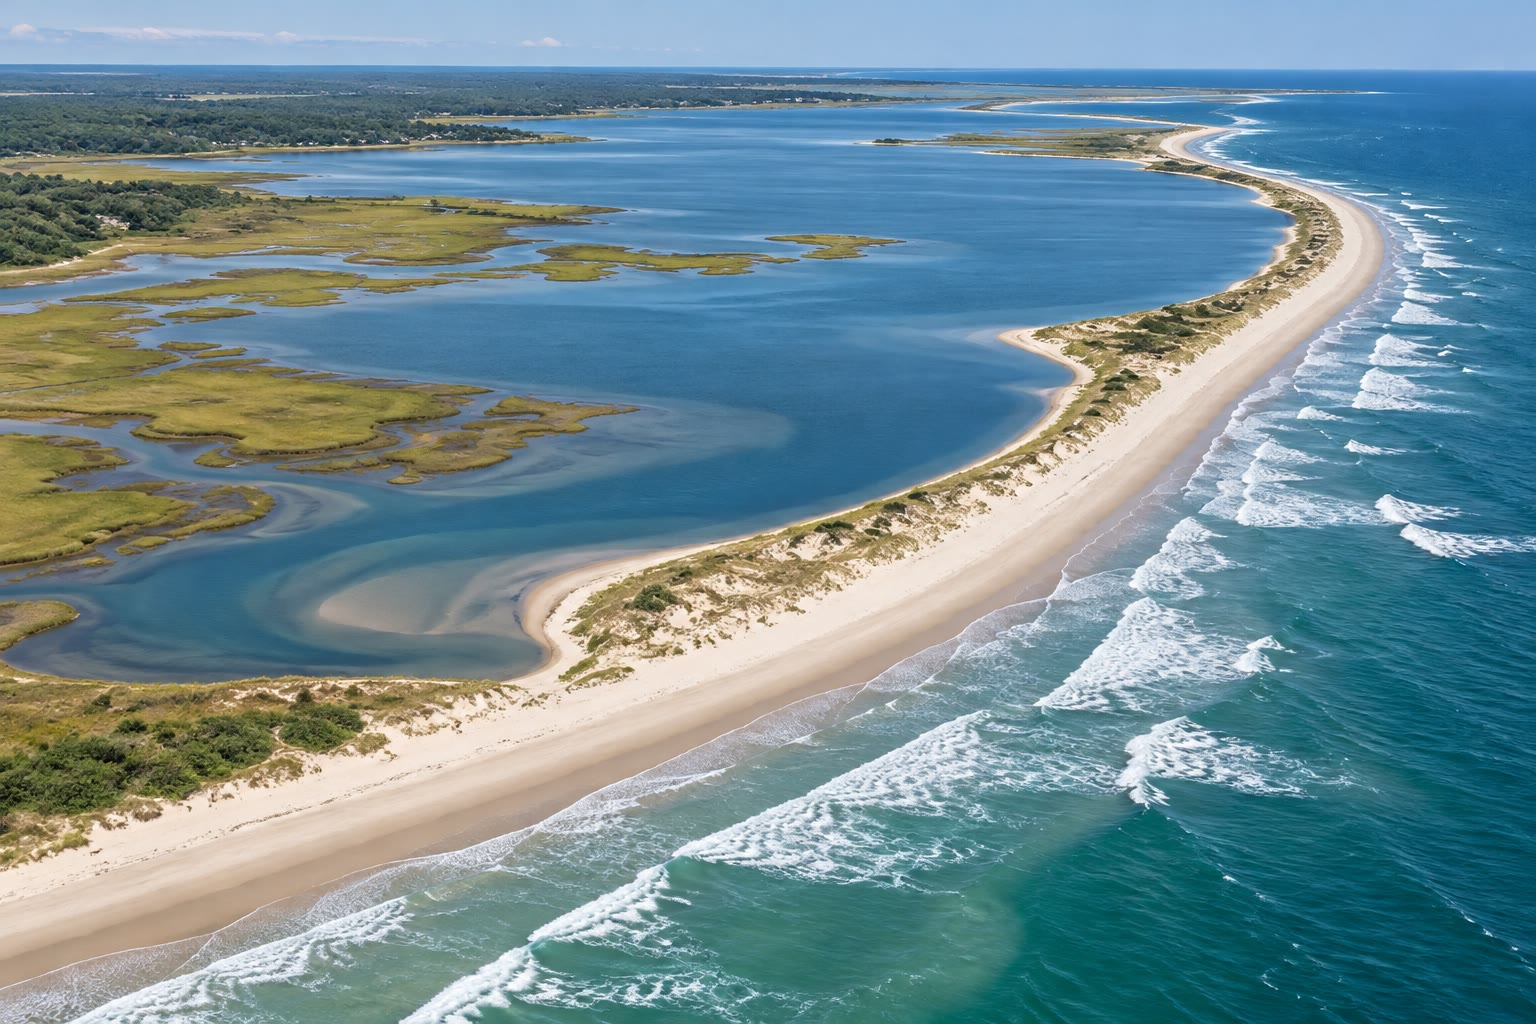
\includegraphics[width=\linewidth]{images/book1/ai/g9-spit-aerial.jpg}
\end{minipage}\hfill
\begin{minipage}[c]{0.46\linewidth}\raggedright
{\small 横跨海湾口的沙质\omterm{def:g9:landforms:beach}{沙嘴}，由低空飞机所摄
（示意图，并非真实地点）。海浪在其面向大海的\omterm{def:g9:landforms:beach}{海滩}上破碎；
其后方是平静的水面与盐沼。}
\end{minipage}
\label{fig:g9:landforms:spit-ai}
\end{omfigure}

\section{溶蚀作用形成的地貌：喀斯特}

雨水并不是纯水。雨水在空中下落，再渗过土壤时，
会吸收二氧化碳，因而略呈酸性。这种弱酸慢慢地
做着稀酸滴在石灰岩上很快便能完成的事，即溶解\omterm{def:g3:stones-pebbles-sand:rock}{岩石}。
石灰岩布满裂隙，既有沿层理的，也有穿过层理的。
水沿这些裂隙渗下，使其变宽，
经数千年，一毫米一毫米地逐步拓宽。
% ledger: usgs:sinkholes, nps:karst

\begin{definition}[喀斯特、洞穴与落水洞]\label{def:g9:landforms:karst}
称\emph{喀斯特}\index{喀斯特}为由水溶解某种可溶性\omterm{def:g3:stones-pebbles-sand:rock}{岩石}所塑造的\omterm{def:g1:landscapes-around-us:landform}{地貌}，
最常见的是石灰岩。那里的\omterm{def:g1:landscapes-around-us:water}{河流}往往潜入地下，
又在别处以泉的形式涌出。\emph{洞穴}\index{洞穴}是
地下足以供人进入的天然空间，
沿\omterm{def:g3:stones-pebbles-sand:rock}{岩石}裂隙溶蚀而成。\emph{落水洞}\index{落水洞}是地表的洼坑
或孔洞，形成于其下方\omterm{def:g3:stones-pebbles-sand:rock}{岩石}被溶蚀掉之处，
或洞穴顶板坍塌之处。
\end{definition}
% ledger: nps:karst, usgs:sinkholes

\begin{omfigure}
\begin{tikzpicture}[x=0.9cm, y=0.9cm, font=\footnotesize, >={Stealth[length=2mm]}]
  \pic (B) at (0,0) {blockdiagram={10}{4}{4}};
  % top face: grassland
  \fill[green!25!black!18] (B-ftl) -- (B-ftr) -- (B-btr) -- (B-btl) -- cycle;
  % right face
  \fill[omLithLime!70] (B-fbr) -- (B-bbr) -- (B-btr) -- (B-ftr) -- cycle;
  % front face: limestone layers
  \fill[omLithLime] (B-fbl) rectangle (B-ftr);
  \foreach \y in {0.8,1.6,2.4,3.2} \draw[black!35] (0,\y) -- (10,\y);
  \foreach \x/\y in {1.2/0.8, 3.1/1.6, 4.6/0, 6.8/2.4, 8.3/0.8, 2.2/2.4, 9.1/2.4, 5.6/3.2}
    \draw[black!35] (\x,\y) -- ++(0,0.8);
  % soil
  \fill[brown!45] (0,3.8) rectangle (10,4);
  % sinkhole on the top face and in the front face
  \fill[green!25!black!35] (3.0,4.45) ellipse (0.7 and 0.22);
  \fill[white] (2.3,4) -- (3.7,4) -- (3.25,3.45) -- (2.75,3.45) -- cycle;
  \fill[green!25!black!30] (2.3,4) -- (3.7,4) -- (3.25,3.45) -- (2.75,3.45) -- cycle;
  \draw[black!60] (2.3,4) -- (2.75,3.45) -- (3.25,3.45) -- (3.7,4);
  % shaft from sinkhole to cave
  \fill[white] (2.85,3.45) -- (3.15,3.45) -- (3.35,2.0) -- (3.05,2.0) -- cycle;
  \draw[black!60] (2.85,3.45) -- (3.05,2.0) (3.15,3.45) -- (3.35,2.0);
  % cave
  \fill[white] (2.6,2.1) .. controls (3.5,2.35) and (5.5,2.3) .. (6.6,1.9)
     .. controls (7.4,1.6) and (7.6,1.2) .. (7.2,1.0)
     .. controls (6.0,0.85) and (4.0,1.0) .. (3.0,1.2)
     .. controls (2.3,1.35) and (2.1,1.9) .. (2.6,2.1) -- cycle;
  \draw[black!70] (2.6,2.1) .. controls (3.5,2.35) and (5.5,2.3) .. (6.6,1.9)
     .. controls (7.4,1.6) and (7.6,1.2) .. (7.2,1.0)
     .. controls (6.0,0.85) and (4.0,1.0) .. (3.0,1.2)
     .. controls (2.3,1.35) and (2.1,1.9) .. (2.6,2.1);
  % underground stream at the cave floor
  \fill[omRiver!60] (3.0,1.2) .. controls (4.0,1.0) and (6.0,0.85) .. (7.2,1.0) -- (7.1,1.12)
     .. controls (6.0,1.0) and (4.0,1.12) .. (3.1,1.3) -- cycle;
  % stalactites and stalagmites
  \foreach \x/\l in {4.2/0.35, 4.5/0.22, 4.9/0.4, 5.3/0.25, 5.8/0.3}
    \fill[black!45] (\x-0.07,2.22) -- (\x+0.06,2.22) -- (\x,2.22-\l) -- cycle;
  \foreach \x/\l in {4.9/0.3, 5.8/0.25}
    \fill[black!45] (\x-0.12,0.95) -- (\x+0.12,0.95) -- (\x,0.95+\l) -- cycle;
  % disappearing stream on the top face
  \draw[omRiver, line width=1.2pt] (7.4,4.85) .. controls (6.9,4.5) and (6.4,4.4) .. (6.0,4.25);
  \fill[black!70] (6.0,4.25) circle (0.07);
  \draw[omRiver, dashed, thick] (6.0,4.0) -- (6.4,2.1);
  % spring on the right face
  \draw[omRiver, line width=1.2pt, ->] (10.2,1.2) .. controls (10.8,1.1) and (11.2,0.7) .. (11.6,0.5);
  % rain with carbon dioxide
  \foreach \x in {0.6,1.2,1.8} \draw[->, omRiver] (\x,5.6) -- ++(-0.15,-0.7);
  \draw[->, omRiver, dashed] (1.0,3.9) -- (1.2,1.7);
  % outline
  \draw[black!70] (B-fbl) rectangle (B-ftr);
  \draw[black!70] (B-ftl) -- (B-btl) -- (B-btr) -- (B-ftr) (B-btr) -- (B-bbr) -- (B-fbr);
  % labels
  \node[anchor=south, align=center] at (1.2,5.6) {雨水吸收二氧化碳 \\而略呈酸性};
  \node[anchor=east, align=right] at (-0.1,1.6) {水使裂隙 \\变宽};
  \draw[black!70] (-0.05,1.6) -- (1.1,2.0);
  \node[anchor=south] at (3.0,5.2) {落水洞};
  \draw[black!70] (3.0,5.2) -- (3.0,4.55);
  \node[anchor=south, align=center] at (7.6,5.3) {河流潜入 \\地下};
  \draw[black!70] (7.0,5.3) -- (6.1,4.35);
  \node[anchor=north, align=center] at (5.0,-0.1) {洞穴：石钟乳自顶板悬垂，\\石笋自地面升起};
  \draw[black!70] (5.0,-0.1) -- (5.0,1.4);
  \node[anchor=west, align=left] at (11.6,0.6) {泉};
  \node[anchor=west] at (11.9,3.4) {石灰岩};
\end{tikzpicture}

{\small \omterm{def:g9:landforms:karst}{喀斯特}\omterm{def:g1:landscapes-around-us:landscape}{景观}（示意图，未按比例）。略带酸性的水
缓缓渗入石灰岩的裂隙并使其变宽；\omterm{def:g6:water-underground:groundwater}{地下
水}流掏蚀出\omterm{def:g9:landforms:karst}{洞穴}；洞顶塌陷形成\omterm{def:g9:landforms:karst}{落水洞}；一
条\omterm{def:g1:landscapes-around-us:water}{河流}潜入洞中，在低处以泉的形式涌出。}
% ledger: nps:karst, usgs:sinkholes, nps:speleothems
\label{fig:g9:landforms:karst}
\end{omfigure}

在\omterm{def:g9:landforms:karst}{洞穴}中，溶解可以逆向进行。一滴水从
洞顶渗下，携带溶解的石灰岩。水滴遇到洞中的
空气时，便释放部分二氧化碳，水滴周围析出一层薄薄的方解石膜。
水滴一滴接一滴，洞顶生出一根空心管，
随后增厚，形成\emph{石钟乳}\index{石钟乳}，状如冰柱悬挂。
水滴落下之处，其余的方解石从地面向上堆起
一座\emph{石笋}\index{石笋}。两者相遇时，
便连成一根石柱。
% ledger: nps:speleothems

\begin{omfigure}
\begin{minipage}[c]{0.5\linewidth}\centering
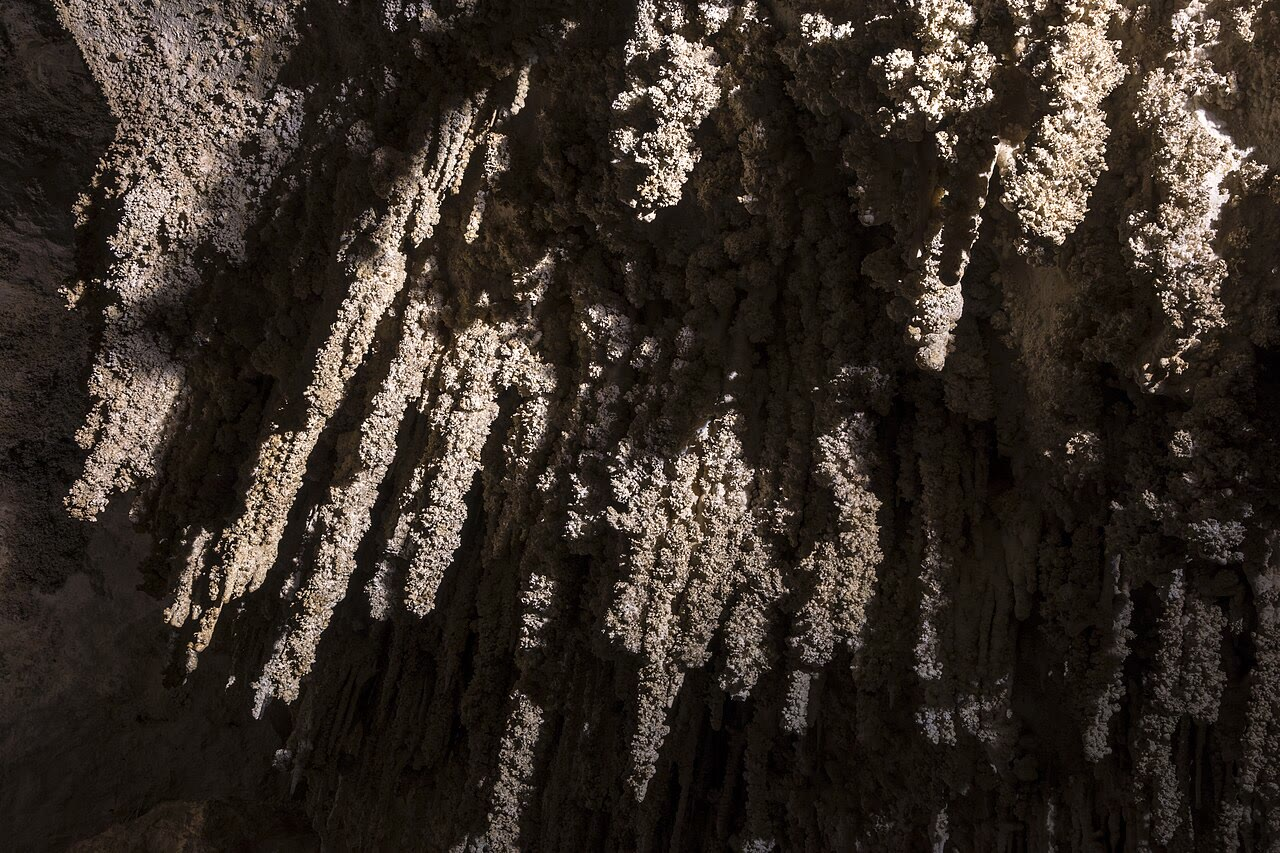
\includegraphics[width=\linewidth]{images/book1/g9-stalactites.jpg}
\end{minipage}\hfill
\begin{minipage}[c]{0.46\linewidth}\raggedright
{\small 卡尔斯巴德\omterm{def:g9:landforms:karst}{洞穴}中，悬挂于一大块\omterm{def:g3:stones-pebbles-sand:rock}{岩石}下的石钟乳，
新墨西哥州的石灰岩溶洞。每一根都是由上方\omterm{def:g3:stones-pebbles-sand:rock}{岩石}渗下的水
滴逐滴堆积而成。National Park Service，2018（公有领域，
经维基共享资源提供）。}
\end{minipage}
% ledger: commons:carlsbad-stalactites, nps:speleothems
\label{fig:g9:landforms:stalactites}
\end{omfigure}

\omterm{def:g9:landforms:karst}{喀斯特}地区地下储水丰富，但水在张开的裂隙中流速很快，
几乎不经过滤：地面上泄漏的任何物质
很快就会到达泉水。下方\omterm{def:g3:stones-pebbles-sand:rock}{岩石}被溶蚀的地方，地面
可能下陷或塌落。在有人居住的地方，突然出现的\omterm{def:g9:landforms:karst}{落水洞}
可能吞没道路与房屋。
% ledger: nps:karst, usgs:sinkholes

\section{解读地貌}

每种\omterm{def:g1:landscapes-around-us:landform}{地貌}都是一条线索：形态说明是哪种营力形成的，营力
说明起作用的过程是\omterm{def:g5:water-shapes-the-land:erosion}{侵蚀}还是\omterm{def:g5:water-shapes-the-land:deposition}{沉积}；而过程
往往能说明下方\omterm{def:g3:stones-pebbles-sand:rock}{岩石}或松散物质的特点。

\begin{method}[识别地貌]
\begin{enumerate}
  \item \textbf{形态。}描述\omterm{def:g1:landscapes-around-us:landform}{地貌}，例如山脊、洼地、陡坡、
        平台；其大小，以及它指向的方向。
  \item \textbf{营力与过程。}判断它是由何种营力形成的（\omterm{def:g1:landscapes-around-us:water}{河流}、
        冰、风、海、溶解作用的水），以及它是经\omterm{def:g5:water-shapes-the-land:erosion}{侵蚀}
        雕刻而成，还是经\omterm{def:g5:water-shapes-the-land:deposition}{沉积}堆积而成。
  \item \textbf{物质。}说明它由什么构成，或下方\omterm{def:g3:stones-pebbles-sand:rock}{岩石}
        可能是什么：松散的沙、\omterm{def:g3:stones-pebbles-sand:pebble}{卵石}、石灰岩，或坚硬或松软的\omterm{def:g3:stones-pebbles-sand:rock}{岩石}。
\end{enumerate}
\end{method}

\begin{center}
{\small
\begin{tabular}{|>{\raggedright\arraybackslash}p{4.6cm}|>{\raggedright\arraybackslash}p{2.6cm}|>{\raggedright\arraybackslash}p{2.2cm}|>{\raggedright\arraybackslash}p{2.6cm}|}
\hline
形态 & 营力 & 过程 & 物质 \\
\hline
新月形\omterm{def:g9:landforms:dune}{沙丘} & 风 & \omterm{def:g5:water-shapes-the-land:deposition}{沉积} & 松散的沙 \\
平坦\omterm{def:g3:stones-pebbles-sand:rock}{岩石}平台上方的竖直岩壁 & 海 & \omterm{def:g5:water-shapes-the-land:erosion}{侵蚀} & \omterm{def:g3:stones-pebbles-sand:rock}{岩石}（软岩后退很快） \\
横跨海湾的狭长沙脊 & 海（\omterm{def:g9:landforms:beach}{沿岸漂移}） & \omterm{def:g5:water-shapes-the-land:deposition}{沉积} & 沙或\omterm{def:g3:stones-pebbles-sand:pebble}{卵石} \\
田野中的洼地、潜入地下的\omterm{def:g1:landscapes-around-us:water}{河流} & 溶解的水 & 溶解 & 石灰岩 \\
\omterm{def:g8:ice-on-earth:glacial-landforms}{U 形谷} & 冰 & \omterm{def:g5:water-shapes-the-land:erosion}{侵蚀} & 任何\omterm{def:g3:stones-pebbles-sand:rock}{岩石} \\
\omterm{def:g5:water-shapes-the-land:source-mouth}{河口}处的泥扇 & \omterm{def:g1:landscapes-around-us:water}{河流} & \omterm{def:g5:water-shapes-the-land:deposition}{沉积} & 泥和沙 \\
\hline
\end{tabular}}
\end{center}

\begin{example}[高原漫步]
在一块长满青草的高原上，地表完全没有\omterm{def:g1:landscapes-around-us:water}{河流}，尽管
这里常常下雨。田野上散布着若干直径仅几米的圆形洼地，而
下方的\omterm{def:g1:landscapes-around-us:landform}{山谷}中，一股强劲的泉水从岩壁脚下涌出。
\emph{形态}：洼地，地表无\omterm{def:g1:landscapes-around-us:water}{河流}，低处有泉。
\emph{营力与过程}：水溶蚀\omterm{def:g3:stones-pebbles-sand:rock}{岩石}，
并在地下流动。\emph{物质}：高原很可能是石灰岩，
洼地即为\omterm{def:g9:landforms:karst}{落水洞}。将一滴稀酸滴在一小块松散的
\omterm{def:g3:stones-pebbles-sand:rock}{岩石}上（由老师放置），会冒泡。
\end{example}
% ledger: nps:karst, usgs:sinkholes

\section{练习}

\begin{exercise}[$\star$]\label{exo:g9:landforms:1}
判断下列每种\omterm{def:g1:landscapes-around-us:landform}{地貌}分别由哪种营力形成：风、海、\omterm{def:g1:landscapes-around-us:water}{河流}、
冰，还是溶解\omterm{def:g3:stones-pebbles-sand:rock}{岩石}的水？(a) \omterm{def:g5:weather-and-climate:desert}{沙漠}中的新月形\omterm{def:g9:landforms:dune}{沙丘}。
(b) 布满石钟乳的\omterm{def:g9:landforms:karst}{洞穴}。(c) 长条\omterm{def:g3:stones-pebbles-sand:pebble}{卵石}脊，横跨
海湾口。(d) 末端带有\omterm{def:g8:ice-on-earth:glacial-landforms}{冰碛}的 \omterm{def:g8:ice-on-earth:glacial-landforms}{U 形谷}。(e) 一面竖直的白垩岩壁，
其底部为平坦的\omterm{def:g3:stones-pebbles-sand:rock}{岩石}平台。(f) 一个\omterm{def:g5:water-shapes-the-land:delta}{三角洲}。
\end{exercise}

\begin{exercise}[$\star$]\label{exo:g9:landforms:2}
写出与下列每条描述对应的术语。(a) 某一地区\omterm{def:g3:stones-pebbles-sand:rock}{岩石}与地面的
缓慢抬升。(b) \omterm{def:g9:landforms:dune}{沙丘}背风一侧的陡坡。
(c) 下方\omterm{def:g3:stones-pebbles-sand:rock}{岩石}溶解或\omterm{def:g9:landforms:karst}{洞穴}顶部塌陷而形成的
地面\omterm{def:g9:landforms:karst}{洞穴}。(d) 沙与\omterm{def:g3:stones-pebbles-sand:pebble}{卵石}沿\omterm{def:g1:landscapes-around-us:water}{海岸}的
移动。(e) 水溶解石灰岩塑造出的\omterm{def:g1:landscapes-around-us:landform}{地貌}。
\end{exercise}

\begin{exercise}[$\star$]\label{exo:g9:landforms:3}
判断正误，并改正错误的句子。(a) 新月形\omterm{def:g9:landforms:dune}{沙丘}的两角
指向风的方向。(b) \omterm{def:g9:landforms:dune}{沙丘}迎风面的坡度
平缓。(c) \omterm{def:g9:landforms:dune}{沙丘}移动是因为风将它整体一次性吹起。(d) \omterm{def:g9:landforms:dune}{沙丘}
在植物稀少的地方更容易形成。
\end{exercise}

\begin{exercise}[$\star$]\label{exo:g9:landforms:4}
将海蚀崖后退的以下步骤按顺序排列。(a) 海浪将
崩落的岩块击碎并搬走。(b) 海浪在崖脚
切出一个缺口。(c) 崖面现在位于更靠内陆的位置，其前方的
平台略微变宽。(d) 缺口上方的\omterm{def:g3:stones-pebbles-sand:rock}{岩石}
向外悬出。(e) 悬出部分坍落。
\end{exercise}

\begin{exercise}[$\star\star$]\label{exo:g9:landforms:5}
% ledger: nps:whsa-migration (6 and 3 m a year)
从飞机上望去，\omterm{def:g5:weather-and-climate:desert}{沙漠}中新月形\omterm{def:g9:landforms:dune}{沙丘}的两角都
指向东方。(a) 风从哪个方向吹来？(b) 每个\omterm{def:g9:landforms:dune}{沙丘}的
\omterm{def:g9:landforms:dune}{滑落面}位于哪一侧？(c) 一条公路位于某个\omterm{def:g9:landforms:dune}{沙丘}东侧 \qty{60}{m} 处，
该\omterm{def:g9:landforms:dune}{沙丘}每年移动 \qty{6}{m}。问经过多少年，它的坡脚将到达公路？
(d) 一个较大的\omterm{def:g9:landforms:dune}{沙丘}每年只移动 \qty{3}{m}。
为什么较大的\omterm{def:g9:landforms:dune}{沙丘}移动得更慢？
\end{exercise}

\begin{exercise}[$\star\star$]\label{exo:g9:landforms:6}
% ledger: sdnp:birling, nt:birling-2014
\omterm{def:g1:landscapes-around-us:water}{海岸}的白垩崖每年最多后退约 \qty{1}{m}。2014 年冬季，
它们在仅两个月内损失的量，相当于通常七年的损失量。
(a) 按每年 \qty{1}{m} 计算，七年共损失多少？
(b) 两个月是一年的几分之几？(c) 这两个月间白垩崖后退的速度
是平时的多少倍？(d) 利用缺口和悬出部分，
解释海崖为何跳跃式后退，
而非平稳后退。
\end{exercise}

\begin{exercise}[$\star\star$]\label{exo:g9:landforms:7}
一段笔直的\omterm{def:g1:landscapes-around-us:water}{海岸}呈西东走向，海位于其南侧。海浪
来自西南方向。(a) \omterm{def:g9:landforms:beach}{沿岸漂移}将沙向哪个方向搬运？
(b) 画出一颗\omterm{def:g3:stones-pebbles-sand:pebble}{卵石}在三次波浪作用下的锯齿形路径，
并标出冲上\omterm{def:g9:landforms:beach}{海滩}和退回的两段路径。(c) \omterm{def:g1:landscapes-around-us:water}{海岸}东端转向北，
进入一个海湾。那里可能会形成什么\omterm{def:g1:landscapes-around-us:landform}{地貌}？
(d) 为什么泥会\omterm{def:g5:water-shapes-the-land:deposition}{沉积}在其后方？
\end{exercise}

\begin{exercise}[$\star\star$]\label{exo:g9:landforms:8}
(a) 是什么使雨水略呈酸性？(b) 为什么石灰岩中有\omterm{def:g9:landforms:karst}{洞穴}，
而花岗岩中几乎没有？(c) 为什么\omterm{def:g9:landforms:karst}{洞穴}沿\omterm{def:g3:stones-pebbles-sand:rock}{岩石}的裂隙和层理发育？
(d) 给出\omterm{def:g9:landforms:karst}{落水洞}形成的两种方式。
\end{exercise}

\begin{exercise}[$\star\star$]\label{exo:g9:landforms:9}
(a) 解释为什么方解石会从\omterm{def:g9:landforms:karst}{洞穴}顶部悬挂的
水滴中析出。(b) 与年轻的钟乳石不同，石笋内部为什么没有
中空的管道？(c) 假设一根钟乳石每年生长 \qty{0.1}{mm}（这是虚构的速率，
实际速率差异很大）。它生长到
\qty{30}{cm} 需要多少年？答案用科学记数法表示。
\end{exercise}

\begin{exercise}[$\star\star$]\label{exo:g9:landforms:10}
% ledger: usgs:himalaya, sdnp:birling
青藏高原在约 1000 万年间\omterm{def:g9:landforms:uplift}{隆升}了约 \qty{4600}{m}。
(a) 计算平均\omterm{def:g9:landforms:uplift}{隆升}速率，分别以米每年（用科学记数法）
和毫米每年表示。(b) 假设\omterm{def:g5:water-shapes-the-land:erosion}{侵蚀}每年从高原上移除 \qty{0.2}{mm}（这是虚构的数值）。
高原每年净抬升多少？(c) 白垩崖每年后退约 \qty{1}{m}。
这比(a)中的\omterm{def:g9:landforms:uplift}{隆升}速率快多少倍？
(d) 为什么缓慢的\omterm{def:g9:landforms:uplift}{隆升}
仍能形成高耸的高原？
\end{exercise}

\begin{exercise}[$\star\star\star$]\label{exo:g9:landforms:11}
用本章的方法（形状、营力与过程、物质）读懂下列\omterm{def:g1:landscapes-around-us:landscape}{景观}。
(a) \omterm{def:g5:natural-hazards:drought}{干旱}地区有成排的新月形\omterm{def:g9:landforms:dune}{沙丘}，
其陡坡一侧朝向东南。(b) 白色\omterm{def:g9:landforms:cliff}{悬崖}脚下，
低潮时，一块覆满海藻的平坦岩台出现。
(c) 在一片宽阔的浅色\omterm{def:g3:stones-pebbles-sand:rock}{岩石}高原上，一条溪流
穿过一片平地后消失于一个洞口；在 \qty{2}{km} 外的
\omterm{def:g1:landscapes-around-us:landform}{山谷}坡面上，有泉水涌出。
\end{exercise}

\begin{exercise}[$\star\star\star$]\label{exo:g9:landforms:12}
% ledger: nps:whsa-migration, nmt:barchan, nps:aeolian
在一片\omterm{def:g9:landforms:dune}{沙丘}区中，迎风边缘的小\omterm{def:g9:landforms:dune}{沙丘}每年最多移动 \qty{6}{m}；
再往前一些，高 6 至 \qty{10}{m} 的\omterm{def:g9:landforms:dune}{沙丘}每年约移动 \qty{3}{m}。
一条小道横穿该\omterm{def:g9:landforms:dune}{沙丘}区，位于每类\omterm{def:g9:landforms:dune}{沙丘}下风方向 \qty{45}{m} 处。
(a) 每个\omterm{def:g9:landforms:dune}{沙丘}经过多少年会到达小道？
(b) 强风驱动的\omterm{def:g9:landforms:dune}{沙丘}一年可移动超过 \qty{100}{m}。这样的\omterm{def:g9:landforms:dune}{沙丘}
走完同样的距离需要多长时间？(c) 说出一种减缓\omterm{def:g9:landforms:dune}{沙丘}移动的方法，
并解释其原理。
\end{exercise}

\section{问题：崖与海岸公路}

\begin{problem}[{周末问题——一条海岸公路位于后退的白垩崖之后，
最终答案是按实测速率，崖边到达公路的
那一年。}]
\label{pb:g9:landforms:1}
% ledger: (invented region: exercise data, figdata/grade-9/cliff_retreat.py; the rate is kept within sdnp:birling, the storm winter recalls nt:birling-2014)
一条\omterm{def:g1:landscapes-around-us:water}{海岸}公路沿白垩崖顶延伸。每隔几年，一支测量队
沿同一条直线测量公路到崖边的距离。
测量点为设在崖边后方的固定标志，从不设在崖边本身。
以下是他们的测量数据。

\begin{center}
{\small
\begin{tabular}{|l|c|c|c|c|c|c|c|}
\hline
年份 & 2004 & 2008 & 2012 & 2014 & 2016 & 2020 & 2024 \\
\hline
公路到崖边的距离 (m) & 46.0 & 43.1 & 41.0 & 36.2 & 35.5 & 33.0 & 30.4 \\
\hline
\end{tabular}}
\end{center}

\noindent\textbf{第一部分——测量数据。}\par\nopagebreak
\begin{enumerate}[beginpenalty=10000]
  \item 2004 年至 2024 年间，崖边
        向公路靠近了多少米？
  \item 计算这 20 年间的平均后退速率，
        以米每年为单位。
  \item 崖边在哪两次测量之间后退最快？计算
        该时段的速率。
  \item 该速率是平均速率的多少倍？推测
        该时段内发生了什么。
\end{enumerate}

\begin{omfigure}
\begin{tikzpicture}
\begin{axis}[omrecord, width=11cm, height=4.6cm, xmin=2000, xmax=2070,
  ymin=0, ymax=50, xtick={2000,2010,...,2070}, ytick={0,10,...,50},
  x tick label style={/pgf/number format/1000 sep={}},
  xlabel={年份}, ylabel={到公路的距离 (m)}]
  \addplot[omWarm, thick, mark=*, mark size=1.8pt] table[x=year, y=dist_m] {figdata/out/grade-9-cliff_retreat.dat};
\end{axis}
\end{tikzpicture}

{\small 调查：从\omterm{def:g1:landscapes-around-us:water}{海岸}公路到崖边的距离（练习
数据）。}
\label{fig:g9:landforms:survey}
\end{omfigure}

\noindent\textbf{第二部分——后退速率。}\par\nopagebreak
\begin{enumerate}[resume, beginpenalty=10000]
  \item 分别以厘米每年和米每世纪为单位，
        写出平均速率。
  \item 在真实的白垩\omterm{def:g1:landscapes-around-us:water}{海岸}上，\omterm{def:g9:landforms:cliff}{悬崖}每年最多后退约一米，
        这座\omterm{def:g9:landforms:cliff}{悬崖}的后退量是否与之相当？
  \item 此类\omterm{def:g1:landscapes-around-us:water}{海岸}上的一座灯塔曾向陆地方向移动了\qty{17}{m}，
        若按这座\omterm{def:g9:landforms:cliff}{悬崖}的平均速率，
        \qty{17}{m}代表多少年的后退？
  \item 为什么用 20 年测得的速率，比两年测得的速率
        更能反映未来的情况？
\end{enumerate}

\noindent\textbf{第三部分——道路。}\par\nopagebreak
\begin{enumerate}[resume, beginpenalty=10000]
  \item 须在崖边距离公路小于\qty{10}{m}之前迁移公路，
        按平均速率，这将发生在哪一年？
  \item 若\omterm{def:g5:natural-hazards:storm}{风暴}更多的冬季使后退速率加倍，崖边将在哪一年
        到达公路？
  \item 测量小组为何要从设在远离崖边处的标桩
        进行测量？
  \item 按平均速率，崖边将在哪一年到达
        公路？
\end{enumerate}
\end{problem}
